\documentclass[]{article}
\usepackage{lmodern}
\usepackage{amssymb,amsmath}
\usepackage{ifxetex,ifluatex}
\usepackage{fixltx2e} % provides \textsubscript
\ifnum 0\ifxetex 1\fi\ifluatex 1\fi=0 % if pdftex
  \usepackage[T1]{fontenc}
  \usepackage[utf8]{inputenc}
\else % if luatex or xelatex
  \ifxetex
    \usepackage{mathspec}
  \else
    \usepackage{fontspec}
  \fi
  \defaultfontfeatures{Ligatures=TeX,Scale=MatchLowercase}
\fi
% use upquote if available, for straight quotes in verbatim environments
\IfFileExists{upquote.sty}{\usepackage{upquote}}{}
% use microtype if available
\IfFileExists{microtype.sty}{%
\usepackage{microtype}
\UseMicrotypeSet[protrusion]{basicmath} % disable protrusion for tt fonts
}{}
\usepackage[margin=1in]{geometry}
\usepackage{hyperref}
\PassOptionsToPackage{usenames,dvipsnames}{color} % color is loaded by hyperref
\hypersetup{unicode=true,
            pdftitle={Hacking for Justice - Introduction to R},
            pdfauthor={Alex C. Engler - The University of Chicago},
            colorlinks=true,
            linkcolor=Maroon,
            citecolor=Blue,
            urlcolor=blue,
            breaklinks=true}
\urlstyle{same}  % don't use monospace font for urls
\usepackage{color}
\usepackage{fancyvrb}
\newcommand{\VerbBar}{|}
\newcommand{\VERB}{\Verb[commandchars=\\\{\}]}
\DefineVerbatimEnvironment{Highlighting}{Verbatim}{commandchars=\\\{\}}
% Add ',fontsize=\small' for more characters per line
\usepackage{framed}
\definecolor{shadecolor}{RGB}{248,248,248}
\newenvironment{Shaded}{\begin{snugshade}}{\end{snugshade}}
\newcommand{\KeywordTok}[1]{\textcolor[rgb]{0.13,0.29,0.53}{\textbf{#1}}}
\newcommand{\DataTypeTok}[1]{\textcolor[rgb]{0.13,0.29,0.53}{#1}}
\newcommand{\DecValTok}[1]{\textcolor[rgb]{0.00,0.00,0.81}{#1}}
\newcommand{\BaseNTok}[1]{\textcolor[rgb]{0.00,0.00,0.81}{#1}}
\newcommand{\FloatTok}[1]{\textcolor[rgb]{0.00,0.00,0.81}{#1}}
\newcommand{\ConstantTok}[1]{\textcolor[rgb]{0.00,0.00,0.00}{#1}}
\newcommand{\CharTok}[1]{\textcolor[rgb]{0.31,0.60,0.02}{#1}}
\newcommand{\SpecialCharTok}[1]{\textcolor[rgb]{0.00,0.00,0.00}{#1}}
\newcommand{\StringTok}[1]{\textcolor[rgb]{0.31,0.60,0.02}{#1}}
\newcommand{\VerbatimStringTok}[1]{\textcolor[rgb]{0.31,0.60,0.02}{#1}}
\newcommand{\SpecialStringTok}[1]{\textcolor[rgb]{0.31,0.60,0.02}{#1}}
\newcommand{\ImportTok}[1]{#1}
\newcommand{\CommentTok}[1]{\textcolor[rgb]{0.56,0.35,0.01}{\textit{#1}}}
\newcommand{\DocumentationTok}[1]{\textcolor[rgb]{0.56,0.35,0.01}{\textbf{\textit{#1}}}}
\newcommand{\AnnotationTok}[1]{\textcolor[rgb]{0.56,0.35,0.01}{\textbf{\textit{#1}}}}
\newcommand{\CommentVarTok}[1]{\textcolor[rgb]{0.56,0.35,0.01}{\textbf{\textit{#1}}}}
\newcommand{\OtherTok}[1]{\textcolor[rgb]{0.56,0.35,0.01}{#1}}
\newcommand{\FunctionTok}[1]{\textcolor[rgb]{0.00,0.00,0.00}{#1}}
\newcommand{\VariableTok}[1]{\textcolor[rgb]{0.00,0.00,0.00}{#1}}
\newcommand{\ControlFlowTok}[1]{\textcolor[rgb]{0.13,0.29,0.53}{\textbf{#1}}}
\newcommand{\OperatorTok}[1]{\textcolor[rgb]{0.81,0.36,0.00}{\textbf{#1}}}
\newcommand{\BuiltInTok}[1]{#1}
\newcommand{\ExtensionTok}[1]{#1}
\newcommand{\PreprocessorTok}[1]{\textcolor[rgb]{0.56,0.35,0.01}{\textit{#1}}}
\newcommand{\AttributeTok}[1]{\textcolor[rgb]{0.77,0.63,0.00}{#1}}
\newcommand{\RegionMarkerTok}[1]{#1}
\newcommand{\InformationTok}[1]{\textcolor[rgb]{0.56,0.35,0.01}{\textbf{\textit{#1}}}}
\newcommand{\WarningTok}[1]{\textcolor[rgb]{0.56,0.35,0.01}{\textbf{\textit{#1}}}}
\newcommand{\AlertTok}[1]{\textcolor[rgb]{0.94,0.16,0.16}{#1}}
\newcommand{\ErrorTok}[1]{\textcolor[rgb]{0.64,0.00,0.00}{\textbf{#1}}}
\newcommand{\NormalTok}[1]{#1}
\usepackage{graphicx,grffile}
\makeatletter
\def\maxwidth{\ifdim\Gin@nat@width>\linewidth\linewidth\else\Gin@nat@width\fi}
\def\maxheight{\ifdim\Gin@nat@height>\textheight\textheight\else\Gin@nat@height\fi}
\makeatother
% Scale images if necessary, so that they will not overflow the page
% margins by default, and it is still possible to overwrite the defaults
% using explicit options in \includegraphics[width, height, ...]{}
\setkeys{Gin}{width=\maxwidth,height=\maxheight,keepaspectratio}
\IfFileExists{parskip.sty}{%
\usepackage{parskip}
}{% else
\setlength{\parindent}{0pt}
\setlength{\parskip}{6pt plus 2pt minus 1pt}
}
\setlength{\emergencystretch}{3em}  % prevent overfull lines
\providecommand{\tightlist}{%
  \setlength{\itemsep}{0pt}\setlength{\parskip}{0pt}}
\setcounter{secnumdepth}{0}
% Redefines (sub)paragraphs to behave more like sections
\ifx\paragraph\undefined\else
\let\oldparagraph\paragraph
\renewcommand{\paragraph}[1]{\oldparagraph{#1}\mbox{}}
\fi
\ifx\subparagraph\undefined\else
\let\oldsubparagraph\subparagraph
\renewcommand{\subparagraph}[1]{\oldsubparagraph{#1}\mbox{}}
\fi

%%% Use protect on footnotes to avoid problems with footnotes in titles
\let\rmarkdownfootnote\footnote%
\def\footnote{\protect\rmarkdownfootnote}

%%% Change title format to be more compact
\usepackage{titling}

% Create subtitle command for use in maketitle
\newcommand{\subtitle}[1]{
  \posttitle{
    \begin{center}\large#1\end{center}
    }
}

\setlength{\droptitle}{-2em}

  \title{Hacking for Justice - Introduction to R}
    \pretitle{\vspace{\droptitle}\centering\huge}
  \posttitle{\par}
    \author{Alex C. Engler - The University of Chicago}
    \preauthor{\centering\large\emph}
  \postauthor{\par}
      \predate{\centering\large\emph}
  \postdate{\par}
    \date{Saturday, September 22nd}


\begin{document}
\maketitle

\subsection{Open RStudio}\label{open-rstudio}

Since you installed R and RStudio during class, you should simply need
to open RStudio (not R) in order to get started. RStudio is a tool to
make working in R (the programming language) a bit easier and more
intuitive.

\subsection{Download the SAO Data}\label{download-the-sao-data}

The State's Attoneys Office (SAO) has four datasets at the case level -
which means each row of data describes one court case. You can find
those datasets
\href{https://datacatalog.cookcountyil.gov/browse?tags=state\%27s\%20attorney\%20case-level}{under
this search on the Cook County Data Catalog}. For your convenience,
direct links to and descriptions of the datasets are provided here:

\begin{itemize}
\tightlist
\item
  \href{https://datacatalog.cookcountyil.gov/Courts/Sentencing/tg8v-tm6u}{Sentencing}:
  The sentencing data presented in this report reflects the judgment
  imposed by the court on people that have been found guilty. Each row
  represents a charge that has been sentenced.
\item
  \href{https://datacatalog.cookcountyil.gov/Courts/Dispositions/apwk-dzx8}{Dispositions}:
  The disposition data presented in this data reflects the culmination
  of the fact-finding process that leads to the resolution of a case.
  Each row represents a charge that has been disposed of.
\item
  \href{https://datacatalog.cookcountyil.gov/Courts/Initiation/7mck-ehwz}{Initiation}:
  The Initiation results data presented here reflects all of the arrests
  that came through the door of the State's Attorneys Office (SAO). An
  initiation is how an arrest turns into a ``case'' in the courts. Most
  cases are initiated through a process known as felony review, in which
  SAO attorneys make a decision whether or not to prosecute. Cases may
  also be indicted by a grand jury or, in narcotics cases, filed
  directly by law enforcement (labeled ``BOND SET (Narcotics)'' in this
  data). Included in this data set are the defendant counts by
  initiation and year. This data includes felony cases handled by the
  Criminal, Narcotics, and Special Prosecution Bureaus. It does not
  include information about cases processed through the Juvenile Justice
  and Civil Actions Bureaus.
\item
  \href{https://datacatalog.cookcountyil.gov/Courts/Intake/3k7z-hchi}{Intake}:
  The intake data presented in this data reflects the cases brought in
  for review. Each row represents a potential defendant in a case.
\end{itemize}

\subsection{Loading Data Into R:}\label{loading-data-into-r}

For our introduction, we will use the tidyverse, which is a set of R
packages that enable quick and (somewhat) intuitive ways to explore and
manipulate date in R. If you have already install the tidyverse using
\texttt{install.packages("tidyverse")}, then you should just need to run
the code below.

\begin{Shaded}
\begin{Highlighting}[]
\KeywordTok{library}\NormalTok{(tidyverse)}
\end{Highlighting}
\end{Shaded}

Next, load the sentencing data into R. The \texttt{read\_csv()} function
loads the data into R, and the assignment operator \texttt{\textless{}-}
saves the data under the name \texttt{sentence}, which we will use to
refer to it from here forward. Data loaded into R is called a
\texttt{dataframe}, and we will use that terminology going forward.

\begin{Shaded}
\begin{Highlighting}[]
\CommentTok{# Note: You can write comments in your R code following a hashtag `#`. }
\CommentTok{# Anything after a hashtag will not run, so you can use comments to write }
\CommentTok{# notes to yourself, explaining what your code does (or should do!).}
\NormalTok{sentence <-}\StringTok{ }\KeywordTok{read_csv}\NormalTok{(}\StringTok{"Sentencing.csv"}\NormalTok{)}
\end{Highlighting}
\end{Shaded}

We can use simple functions, like \texttt{nrow()} and \texttt{ncol} to
see how many rows and columns of data there are in this dataframe. Note,
you must use all lowercase letters for \texttt{sentence} and the
function names, as R is case sensitive.

\begin{Shaded}
\begin{Highlighting}[]
\KeywordTok{nrow}\NormalTok{(sentence)}
\end{Highlighting}
\end{Shaded}

\begin{verbatim}
## [1] 189287
\end{verbatim}

\begin{Shaded}
\begin{Highlighting}[]
\KeywordTok{ncol}\NormalTok{(sentence)}
\end{Highlighting}
\end{Shaded}

\begin{verbatim}
## [1] 36
\end{verbatim}

We can visually inspect our loaded dataframe with the \texttt{glimpse()}
function. This prints each column, or variable, in the dataset on each
row. It also tells us what type of variable is contained in the column
(e.g.~a \texttt{dbl} means a continuous number, whereas a \texttt{chr}
means characters, which could be letters, numbers or a sentence).
Finally, this function shows us some of the first values in each column,
listed from left to right.

\begin{Shaded}
\begin{Highlighting}[]
\KeywordTok{glimpse}\NormalTok{(sentence)}
\end{Highlighting}
\end{Shaded}

\begin{verbatim}
## Observations: 189,287
## Variables: 36
## $ CASE_ID                   <dbl> 26783584167, 26651437018, 2676852092...
## $ CASE_PARTICIPANT_ID       <dbl> 46480038575, 46118600972, 4643960910...
## $ CHARGE_ID                 <dbl> 33613165290, 33297012068, 3361328199...
## $ CHARGE_VERSION_ID         <dbl> 200413732973, 200414312333, 20041445...
## $ PRIMARY_CHARGE            <chr> "true", "true", "true", "false", "tr...
## $ OFFENSE_TITLE             <chr> "UNLAWFUL USE OR POSSESSION OF A WEA...
## $ CHAPTER                   <chr> "720", "720", "720", "720", "720", "...
## $ ACT                       <int> 5, 570, 5, 550, 570, 5, 5, 5, 570, 5...
## $ SECTION                   <chr> "24-1.1(a)", "402(c)", "19-1(a)", "4...
## $ CLASS                     <chr> "2", "4", "2", "4", "4", "2", "2", "...
## $ AOIC                      <chr> "0012309", "5101110", "1110000", "50...
## $ DISPO_DATE                <chr> "10/11/2012 12:00:00 AM", "07/29/201...
## $ SENTENCE_PHASE            <chr> "Original Sentencing", "Original Sen...
## $ SENTENCE_DATE             <chr> "10/03/2012 12:00:00 AM", "07/28/201...
## $ SENTENCE_JUDGE            <chr> "Stanley  Sacks", "Thaddeus L Wilson...
## $ SENTENCE_TYPE             <chr> "Prison", "Probation", "Prison", "Pr...
## $ COMMITMENT_TYPE           <chr> "Illinois Department of Corrections"...
## $ COMMITMENT_TERM           <dbl> 6, 2, 6, 2, 2, 7, 3, 16, 3, 2, 2, 1,...
## $ COMMITMENT_UNIT           <chr> "Year(s)", "Year(s)", "Year(s)", "Ye...
## $ CHARGE_DISPOSITION        <chr> "Plea Of Guilty", "Plea Of Guilty", ...
## $ CHARGE_DISPOSITION_REASON <chr> NA, NA, NA, NA, NA, NA, NA, NA, NA, ...
## $ COURT_NAME                <chr> "District 1 - Chicago", "District 1 ...
## $ COURT_FACILITY            <chr> "26TH Street", "26TH Street", "26TH ...
## $ LENGTH_OF_CASE_in_Days    <int> 414, 86, 339, 86, 44, 31, NA, 709, 1...
## $ AGE_AT_INCIDENT           <int> 29, 45, 50, 45, 41, 25, 30, 19, 57, ...
## $ GENDER                    <chr> "Male", "Male", "Male", "Male", "Mal...
## $ RACE                      <chr> "Black", "HISPANIC", "Black", "HISPA...
## $ OFFENSE_TYPE              <chr> "UUW - Unlawful Use of Weapon", "Nar...
## $ INCIDENT_BEGIN_DATE       <chr> "07/06/2011 12:00:00 AM", "03/26/201...
## $ INCIDENT_END_DATE         <chr> NA, NA, NA, NA, NA, NA, NA, NA, NA, ...
## $ ARREST_DATE               <chr> "07/06/2011 11:35:00 PM", "03/26/201...
## $ LAW_ENFORCEMENT_AGENCY    <chr> "CHICAGO PD", "CHICAGO PD", "CHICAGO...
## $ UNIT                      <chr> "District 10 - Ogden", "District 8 -...
## $ INCIDENT_CITY             <chr> "Chicago", "Chicago", "Chicago", "Ch...
## $ RECEIVED_DATE             <chr> "07/07/2011 12:00:00 AM", "03/29/201...
## $ ARRAIGNMENT_DATE          <chr> "08/16/2011 12:00:00 AM", "05/03/201...
\end{verbatim}

\pagebreak

Some of the data is self-explanatory, for instance, the
\texttt{SENTENCE\_TYPE} column contains the type of the sentence that
resulted in this judgement. Below, we use the \texttt{table()} function
to create a frequency table - this tells us every value of the
\texttt{SENTENCE\_TYPE} column and how many times that value appears in
the dataset. We use the \texttt{\$} operator to refer to the
\texttt{SENTENCE\_TYPE} column within the \texttt{sentence} dataframe.

\begin{Shaded}
\begin{Highlighting}[]
\KeywordTok{table}\NormalTok{(sentence}\OperatorTok{$}\NormalTok{SENTENCE_TYPE)}
\end{Highlighting}
\end{Shaded}

\begin{verbatim}
## 
##                  2nd Chance Probation 
##                                  1080 
##                 Conditional Discharge 
##                                  2696 
##                   Conditional Release 
##                                    70 
##                            Conversion 
##                                     5 
##                 Cook County Boot Camp 
##                                  1806 
##                                 Death 
##                                    59 
##      Inpatient Mental Health Services 
##                                   137 
##                                  Jail 
##                                  5563 
##                                Prison 
##                                106093 
##                             Probation 
##                                 69499 
##        Probation Terminated Instanter 
##                                    74 
##   Probation Terminated Satisfactorily 
##                                    43 
## Probation Terminated Unsatisfactorily 
##                                   569 
##                           Supervision 
##                                  1593
\end{verbatim}

\begin{Shaded}
\begin{Highlighting}[]
\CommentTok{# or count(sentences, SENTENCE_TYPE)}
\end{Highlighting}
\end{Shaded}

\subsubsection{Remember to Use the Data
Documentation}\label{remember-to-use-the-data-documentation}

However, other columns may not be so easily interpreted, and guessing
can lead to mistakes. For instance, the \texttt{PRIMARY\_CHARGE} column
has values of ``true'' and ``false'', which is not clearly
self-explanatory.

It's important to consistently use the data documentation, sometimes
called a codebook, to help learn about a dataset. Scrolling down on the
\href{https://datacatalog.cookcountyil.gov/Courts/Sentencing/tg8v-tm6u}{same
page we found this data}, we can see there are short descriptions of
what each coulmn contains.

\begin{Shaded}
\begin{Highlighting}[]
\KeywordTok{table}\NormalTok{(sentence}\OperatorTok{$}\NormalTok{PRIMARY_CHARGE)}
\end{Highlighting}
\end{Shaded}

\begin{verbatim}
## 
##  false   true 
##  50411 138876
\end{verbatim}

\begin{Shaded}
\begin{Highlighting}[]
\CommentTok{# or count(sentences, PRIMARY_CHARGE)}
\end{Highlighting}
\end{Shaded}

\subsection{Level Of The Data}\label{level-of-the-data}

Reading the documentation has revealed something important about the
data (as it often does!). It is easy to open this dataset and assume
that each row of data was the sentencing for a distinct and unique case.
However, this is not correct! We can see there are many cases that
appear in the data more than once.

Below, we first create a list of all distinct values of the
\texttt{CASE\_ID} column using the \texttt{unique()} function. Then, in
the same line of code, we count how many there are using
\texttt{length()}.

\begin{Shaded}
\begin{Highlighting}[]
\KeywordTok{length}\NormalTok{(}\KeywordTok{unique}\NormalTok{(sentence}\OperatorTok{$}\NormalTok{CASE_ID))}
\end{Highlighting}
\end{Shaded}

\begin{verbatim}
## [1] 155443
\end{verbatim}

This results in 155443 unique values, far fewer than the 189287 rows of
data.

\subsubsection{Breaking Apart Confusing
Code}\label{breaking-apart-confusing-code}

If the code above was tough for you to follow, try break it apart into
its component pieces. For instance, what happens if you just run the
following line:

\begin{verbatim}
unique(c("cat", "dog", "fish, "cat))
\end{verbatim}

Does this help better illustrate how \texttt{unique()} is working? Now
trying running \texttt{length()} and \texttt{unique()} together, like
below.

\begin{verbatim}
length(unique(c("cat", "dog", "fish, "cat)))
\end{verbatim}

\subsubsection{Interpreting the Level Of the
Data}\label{interpreting-the-level-of-the-data}

In this data, one row is actually defined by the \texttt{CHARGE\_ID}
variable. This is to say that each row of data, or observation, is one
unique charge resulting in sentencing, with potentially several or many
charges per case.

This is important, since if we were to simply look at the average age
across this dataset, we might substantially misinterpret the resulting
number. Instead, lets select a group of columns that will be consistent
across each case. Below, we use the \texttt{select()} function to grab
only a few of the columns.

\subsubsection{Columnar Selection}\label{columnar-selection}

\begin{Shaded}
\begin{Highlighting}[]
\NormalTok{cases <-}\StringTok{ }\KeywordTok{select}\NormalTok{(sentence, CASE_ID, CASE_PARTICIPANT_ID, AGE_AT_INCIDENT, GENDER, RACE, LENGTH_OF_CASE_in_Days)}
\KeywordTok{dim}\NormalTok{(cases) }\CommentTok{# See the number of rows, columns in the data}
\end{Highlighting}
\end{Shaded}

\begin{verbatim}
## [1] 189287      6
\end{verbatim}

\subsubsection{}\label{section}

\begin{Shaded}
\begin{Highlighting}[]
\NormalTok{cases <-}\StringTok{ }\KeywordTok{distinct}\NormalTok{(cases)}
\KeywordTok{dim}\NormalTok{(cases)}
\end{Highlighting}
\end{Shaded}

\begin{verbatim}
## [1] 167397      6
\end{verbatim}

\begin{Shaded}
\begin{Highlighting}[]
\KeywordTok{mean}\NormalTok{(cases}\OperatorTok{$}\NormalTok{AGE_AT_INCIDENT)}
\end{Highlighting}
\end{Shaded}

\begin{verbatim}
## [1] NA
\end{verbatim}

\begin{Shaded}
\begin{Highlighting}[]
\KeywordTok{median}\NormalTok{(cases}\OperatorTok{$}\NormalTok{LENGTH_OF_CASE_in_Days)}
\end{Highlighting}
\end{Shaded}

\begin{verbatim}
## [1] NA
\end{verbatim}

\begin{Shaded}
\begin{Highlighting}[]
\KeywordTok{table}\NormalTok{(cases}\OperatorTok{$}\NormalTok{RACE)}
\end{Highlighting}
\end{Shaded}

\begin{verbatim}
## 
##                  American Indian                            Asian 
##                               92                              969 
##                            ASIAN                         Biracial 
##                               51                               31 
##                            Black                         HISPANIC 
##                           110498                             4512 
##                          Unknown                            White 
##                              228                            24525 
##       White [Hispanic or Latino] White/Black [Hispanic or Latino] 
##                            24748                              812
\end{verbatim}

\begin{Shaded}
\begin{Highlighting}[]
\KeywordTok{prop.table}\NormalTok{(}\KeywordTok{table}\NormalTok{(cases}\OperatorTok{$}\NormalTok{GENDER))}
\end{Highlighting}
\end{Shaded}

\begin{verbatim}
## 
##                     Female                       Male 
##               1.269817e-01               8.729704e-01 
## Male name, no gender given                    Unknown 
##               1.798777e-05               2.398369e-05 
##             Unknown Gender 
##               5.995923e-06
\end{verbatim}

\subsubsection{Grouped Aggregation}\label{grouped-aggregation}

Let's

cases \textless{}- group\_by(sentence, CASE\_ID) summarize(cases,
avg\_age = mean(AGE\_AT\_INCIDENT), count=n())

\subsection{We can see more charges per person at younger ages, so our
original histogram was skewed to the
left.}\label{we-can-see-more-charges-per-person-at-younger-ages-so-our-original-histogram-was-skewed-to-the-left.}

sentence \%\textgreater{}\% group\_by(CASE\_ID) \%\textgreater{}\%
summarize(age = mean(AGE\_AT\_INCIDENT), count=n()) \%\textgreater{}\%
ggplot(aes(age, count)) + geom\_point()

sentence \%\textgreater{}\% group\_by(CASE\_ID, AGE\_AT\_INCIDENT)
\%\textgreater{}\% summarize(count=n()) \%\textgreater{}\% filter(count
\textless{} 15) \%\textgreater{}\% ggplot(aes(count)) +
geom\_histogram()

\begin{Shaded}
\begin{Highlighting}[]
\KeywordTok{hist}\NormalTok{(sentence}\OperatorTok{$}\NormalTok{AGE_AT_INCIDENT)}
\end{Highlighting}
\end{Shaded}

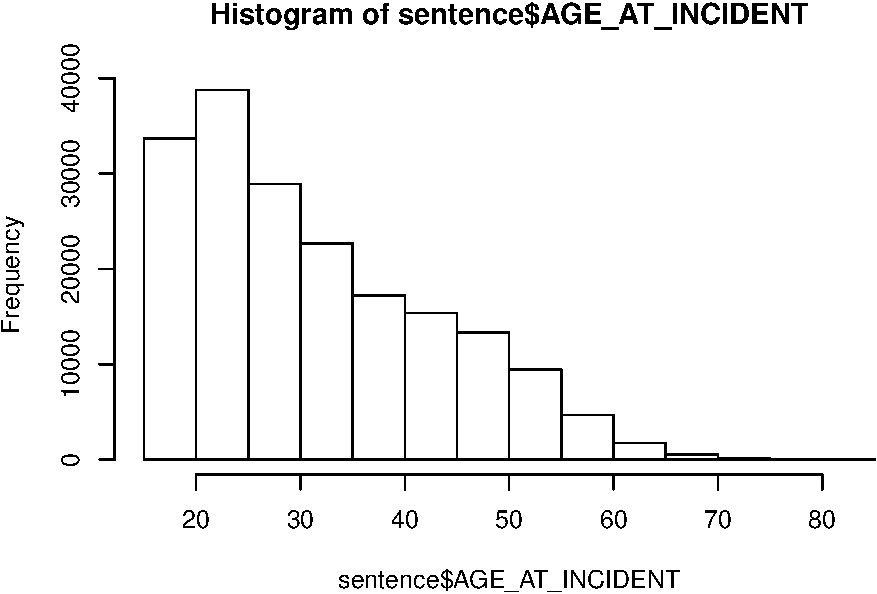
\includegraphics{HFJ-RStats_files/figure-latex/unnamed-chunk-11-1.pdf}

\begin{Shaded}
\begin{Highlighting}[]
\CommentTok{# Or}
\CommentTok{# ggplot(sentence, aes(AGE_AT_INCIDENT)) + geom_histogram()}
\end{Highlighting}
\end{Shaded}

\subsection{Filtering The Data}\label{filtering-the-data}

We can use the \texttt{filter()} function to look at only some rows of
the data. Below, I have created several smaller datasets from the
original. Each new dataset, on the left of the assignment operator
\texttt{\textless{}-} is composed of the rows from the original dataset
that meet the criteria specified in the \texttt{filter()\ function}.

\begin{Shaded}
\begin{Highlighting}[]
\NormalTok{sentence_female <-}\StringTok{ }\KeywordTok{filter}\NormalTok{(sentence, GENDER }\OperatorTok{==}\StringTok{ "Female"}\NormalTok{) ## == means exactly equal to}
\NormalTok{sentence_under21 <-}\StringTok{ }\KeywordTok{filter}\NormalTok{(sentence, AGE_AT_INCIDENT }\OperatorTok{<=}\StringTok{ }\DecValTok{21}\NormalTok{) ## <= means less than or equal to}
\CommentTok{#sentence_probation <- filter(sentence, SENTENCE_TYPE %in% c("Probation", "2nd Chance Probation")) ## %in% means 'is one of'}
\end{Highlighting}
\end{Shaded}

How can you be sure that these filters worked as you expected? Use the
\texttt{table()} function and the \texttt{hist()} function on the newly
created datasets (sentence\_female, sentence\_under21, and
sentence\_probation) to ensure you understand what the filters
accomplished.

If you were able to confirm what was happening above, try this on your
own. Write a filter that only looks at cases longer than one year (using
\texttt{LENGTH\_OF\_CASE\_in\_Days}) and/or sentencing imposed on
Hispanic persons.

\pagebreak

\subsection{Merging On Another
Dataset}\label{merging-on-another-dataset}

Let's load in a different dataset from the SAO:

\begin{Shaded}
\begin{Highlighting}[]
\NormalTok{initiation <-}\StringTok{ }\KeywordTok{read_csv}\NormalTok{(}\StringTok{"Initiation.csv"}\NormalTok{)}
\end{Highlighting}
\end{Shaded}

Always make sure to carefully examine new datasets. This should at least
including using functions like \texttt{glimpse()} or \texttt{View()} to
look at the data, as well as explorations we have used today like
\texttt{table()}, \texttt{hist()}, and \texttt{unique()}.

\pagebreak

\subsection{Appendix 1: R Terminology}\label{appendix-1-r-terminology}

\begin{itemize}
\tightlist
\item
  Comments: Everything after a \texttt{\#} (a hashtag) in your code will
  have no effect if you run it in R. Thus, you can use \texttt{\#}
  hashtags to write notes to yourself and others, making your code more
  readable.
\item
  Working Directory : The folder on your computer that R is currently
  working in. It will only check this folder for files to load, and will
  write any new files to this folder.
\item
  Dataframe : the R equivalent of an excel file. It holds relational
  data in rows and columns that can contain numbers or strings.
\item
  Assignment Operator \texttt{\textless{}-} : Gives the value on the
  right to the object on the left.
\item
  Function : Anything that completes a task or set of tasks in R is a
  function. Most functions have a name, and take one or more arguments
  within parentheses. Examples include `head()', `colnames()', `hist()',
  `mean()', `and plot()'\\
\item
  Argument : An input or an option that affects the result of a
  function. This often includes the data that the function runs on, AND
  specifications/options as to what the function should do. For example:
\end{itemize}

\texttt{hist(dataframe\$column,\ main\ =\ "A\ Histogram")}

The function above (hist is a function for making a histogram) above is
given two arguments, separated by a comma. The first is `data\$column',
telling the histogram to use the data in this column to make a
histogram. The second arguments is `main = ``A Histogram''\,', which is
activating an option, and giving the histogram a main title.

\subsubsection{Mathematical Operators in
R:}\label{mathematical-operators-in-r}

\begin{Shaded}
\begin{Highlighting}[]
\DecValTok{2}\OperatorTok{+}\DecValTok{2} \CommentTok{# Addition with the plus sign `+`}
\end{Highlighting}
\end{Shaded}

\begin{verbatim}
## [1] 4
\end{verbatim}

\begin{Shaded}
\begin{Highlighting}[]
\DecValTok{6}\OperatorTok{-}\DecValTok{3} \CommentTok{# Subtraction with the - sign}
\end{Highlighting}
\end{Shaded}

\begin{verbatim}
## [1] 3
\end{verbatim}

\begin{Shaded}
\begin{Highlighting}[]
\DecValTok{4}\OperatorTok{*}\DecValTok{2} \CommentTok{# The asterisk (*) indicates multiplication}
\end{Highlighting}
\end{Shaded}

\begin{verbatim}
## [1] 8
\end{verbatim}

\begin{Shaded}
\begin{Highlighting}[]
\DecValTok{12}\OperatorTok{/}\DecValTok{3} \CommentTok{# Division usses the backslash}
\end{Highlighting}
\end{Shaded}

\begin{verbatim}
## [1] 4
\end{verbatim}

\begin{Shaded}
\begin{Highlighting}[]
\DecValTok{3}\OperatorTok{^}\DecValTok{3}\NormalTok{ ## This caret `^` means exponentiation, so this is 3 to the third power.}
\end{Highlighting}
\end{Shaded}

\begin{verbatim}
## [1] 27
\end{verbatim}

\pagebreak 

\subsection{Appendix 2: Pertinent
Resources}\label{appendix-2-pertinent-resources}

\textbf{Introduction to haven package}
\href{https://blog.rstudio.org/2015/03/04/haven-0-1-0/}{Link}

\textbf{Introduction to readr package}
\href{https://github.com/tidyverse/readr}{Link}

\textbf{Introduction to readxl package}
\href{https://github.com/tidyverse/readxl}{Link}

\textbf{Vignette on dplyr package for Data Manipulation}
\href{https://cran.rstudio.com/web/packages/dplyr/vignettes/introduction.html}{Link}

\textbf{Data Processing with dplyr \& tidyr}
\href{https://rpubs.com/bradleyboehmke/data_wrangling}{Link}

\textbf{String Manipulation with stringr}
\href{https://cran.r-project.org/web/packages/stringr/vignettes/stringr.html}{Link}

\begin{center}\rule{0.5\linewidth}{\linethickness}\end{center}

In the image above {[}Figure 1{]}, you can see how to navigate to the
RStudio Cheat Sheets for R's very useful data manipulation packages,
\texttt{dplyr} and \texttt{tidyr}. These packages, as well as
\texttt{stringr}, are also covered in detail in the excellent free ebook
\href{http://r4ds.had.co.nz/transform.html}{R for Data Science}.

\begin{figure}
\centering
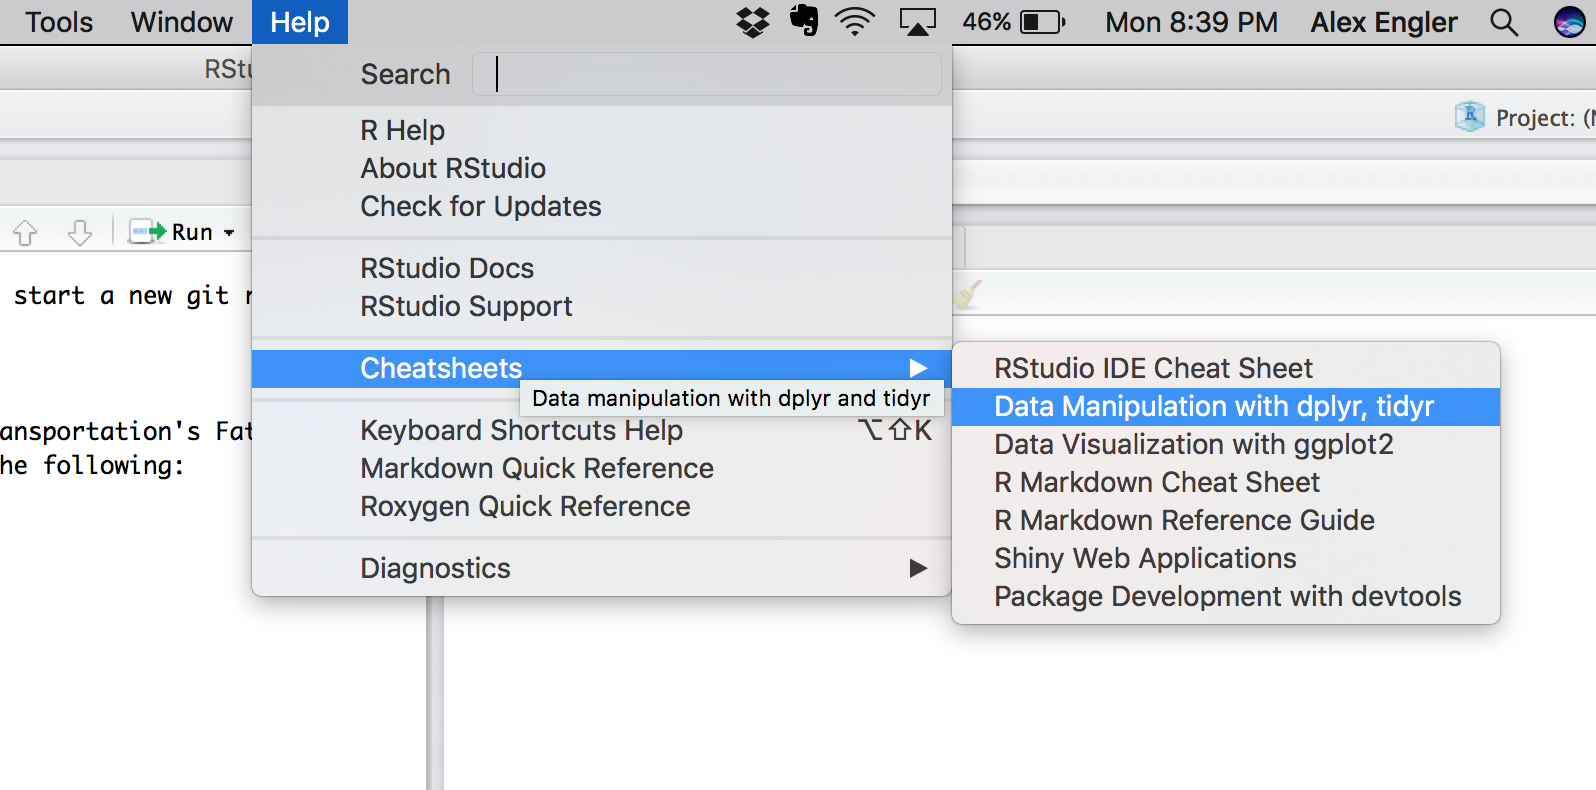
\includegraphics{./cheat.png}
\caption{Cheat Sheets}
\end{figure}


\end{document}
